\providecommand{\keywords}[1]{\textbf{\textit{Keywords.}} #1}

\chapter{Literature Review} \label{chap:literature-review}
\keywords{artificial intelligence, stock market}
\section{Introduction}
As the world advances in technology, an increasing number of decisions are dependent on computational models; including financial decisions. This includes, but is not limited to, decisions for money management, risk management, economics, and investing.
This literature review will discuss: the feasibility of predicting stock market prices; different artificial intelligence research methods used in financial modelling, particular those that relate to investing and stock market indices; and the different input features used in these models.

\section{Feasibility of predicting stock market index prices}
\subsection{Efficient Market Hypothesis}
Over the year,  many people have attempted to predict stock markets in order to profit from price movements as they occur. However, some have theorised that it is not possible to accurately predict prices due to the there being an innumerable number of factors that can affect a stock market, and these factors would already be a function of the current market's price, therefore make it impossible to forecast the price. \parencite[1]{theoryofspeculation} This is the basis of the Efficient Market Hypothesis, where an asset price fully reflects the information that is available at any given time.

\subsection{Empirical evidence of market (in)efficiencies}
A 1973 book explains the term `random walk' as ``A random walk is one in which future steps or directions cannot be predicted on the basis of past actions``, and continues to describe how when applied to the stock market that ``short-run changes in stock prices are unpredictable. [and] Investment advisory services, earnings forecasts, and complicated chart patterns are useless'' \parencite[24]{burton_gordon_malkiel_2016}.
A reflection paper by the same author 30 years on, attempts to validate that the efficient market hypothesis still holds true in the 21st century by comparing actively managed funds to tracker funds: suggesting that markets are likely efficient, due to the fact that most actively managed funds are outperformed by a index tracker fund that follows the S\&P 500 index; the data presented suggests that most experts (68\% to 90\% over various time periods) cannot outperform the index whether it be from a one year, three year, five year, ten year or twenty year holding period leading up to 31st December, 2003 \parencite{reflections30years}. The author suggests that if markets were inefficient, fund managers should easily be able to outperform the index.

In order to prove, or disprove, the Efficient Market Hypothesis, many studies have been carried out with varying results. In this literature review we will focus on the US markets and the different results the studies have found. Using data from 1964 to 2003 for the US stock market, one study has found markets to be efficient using a threshold autoregressive model and a unit root process \parencite{narayan2006behaviour}. Another empirical look into equity premium prediction, that looks specifically at the US S\&P 500 index, using various regression models with additional variables described such as dividends, earnings price ratio, book value, net issuing activity and more has concluded that ``the equity premium has not been predictable'' \parencite[abstract]{goval_welch_2004} which would agree with the efficient market hypothesis.

% A study with a more up-to-date dataset, that looks at 350 companies listed on the London Stock Exchange and S\&P 500 between 2007 to 2013, using an auto-regressive moving average model can be used to calculate mid-long term returns on the LSE and monthly/annual on SP500. https://doi.org/10.1016/j.physa.2016.03.006

However, other recent studies have suggested the efficient market hypothesis may not hold true. A paper that looks into returns of the US Dow Jones Industrial Average (DJIA) index from 1928 to 2012 showed that while for autocorrelation tests on daily and weekly intervals suggest market efficiency, the same cannot be said for monthly and annual intervals (although the degree of correlation is low). Furthermore, the paper posits that autocorrelation tests are not sufficient to determine dependencies, and puts forwards another type of test called `run tests' to show that markets are also inefficient in daily and weekly intervals \parencite{sewell_2012}. Another paper that analyses data from 1999 to 2007 of various markets, including the US as well as other developed and developing countries, using a unit root process has stated that their findings show that ``real stock price indices are stationary processes that are inconsistent with the efficient market hypothesis'' \parencite[1]{LEE201049}.

%file:///C:/Users/alvie/Downloads/IJMFA70307_Rossi_LR_CA3.pdf

%https://etalpykla.lituanistikadb.lt/object/LT-LDB-0001:J.04~2015~1447771572718/J.04~2015~1447771572718.pdf


\section{Types of artificial intelligence methods used}

\subsection{Description of artificial intelligence methods}
Various artificial intelligence methods have been utilised in order to predict daily direction as well
as price of stock markets, the following are described here:
\begin{itemize}
    \item Multilayer Perceptrons (MLPs)
    \item Convolutional Neural Networks (CNNs)
    \item Support Vector Machines (SVMs)
    \item Long Short Term Memory (LSTM)
    \item Hybrid approaches
\end{itemize}

\subsubsection{Multilayer Perceptrons (MLPs)}
Multilayer Perceptrons (MLPs - \autoref{fig:multilayer-perceptron}) are a class of artificial neural networks. They contain multiple layers
of perceptrons, including an input layer, one or many hidden layers and an output layer. They are
feed-forward networks meaning that data is only passed to the next layer and does not move backwards.
It is an example of a supervised neural network as labelled data is used in training.

\begin{figure}[hbt!]
    \centering
    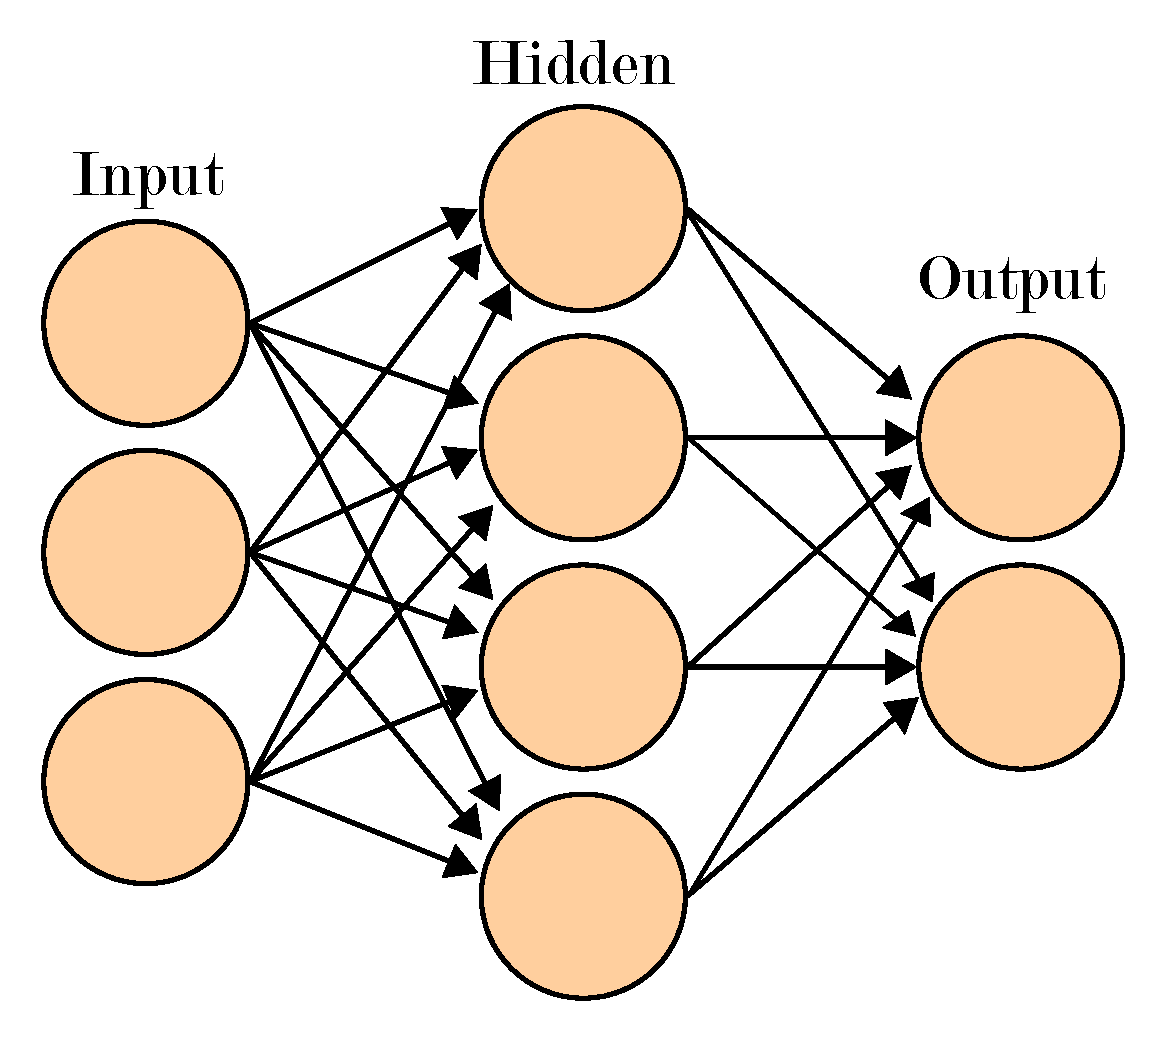
\includegraphics[width=0.4\columnwidth]{figures/multilayer-perceptron.pdf}
    \caption[Diagram of a Multilayer Perceptron]{Diagram of a Multilayer Perceptron; adapted from Artificial neural network.svg, Wikimedia, Cburnett}
    \label{fig:multilayer-perceptron}
\end{figure}
\FloatBarrier

\subsubsection{Convolutional Neural Networks (CNNs)}
Convolutional Neural Networks (CNNs - \autoref{fig:convolutional-neural-network}) are a class of artificial neural networks. They contain
multiple layers; including an input layer, one or many convolutional and pooling layers, and an
output layer. The convolutional and pooling layers are inspired by biological processes; each
layer extracts and summarises certain features and convolves the input and passes to the next
layer. The pooling layers are using to reduce the spatial size of the data by combining outputs
in order to optimise the network for performance.

They are feed-forward networks meaning that data is only passed to the next layer and does
not move backwards. It is an example of a supervised neural network as labelled data is used
in training.

\begin{figure}[hbt!]
    \centering
    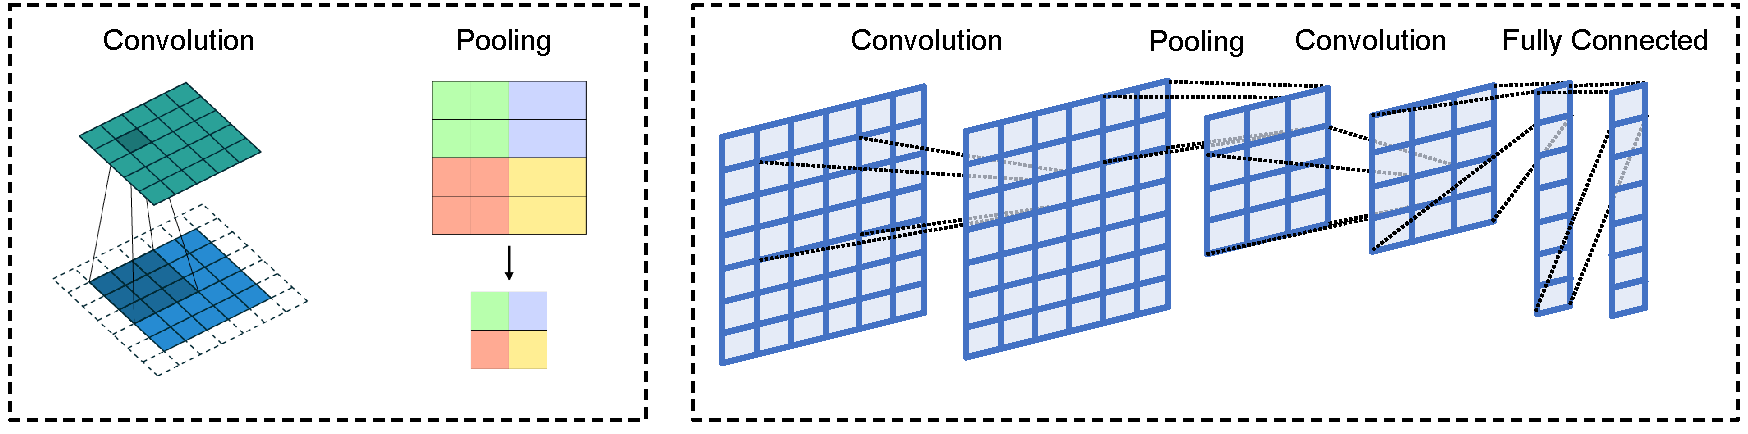
\includegraphics[width=0.75\columnwidth]{figures/convolutional-neural-networks.pdf}
    \caption[Diagram of a Convolutional Neural Network]{Diagram of a Convolutional Neural Network; \parencite{Maier2019}}
    \label{fig:convolutional-neural-network}
\end{figure}
\FloatBarrier

\subsubsection{Support Vector Machines (SVM)}
Support Vector Machines (SVMs - \autoref{fig:support-vector-machines}) are a class of machine learning models that are used in classification
of data. In this model, the training data is used in order to identify a decision boundary, known as
a hyperplane that separates the classifications of data. It is an example of a supervised machine
learning model as labelled data is used in training.
\begin{figure}[hbt!]
    \centering
    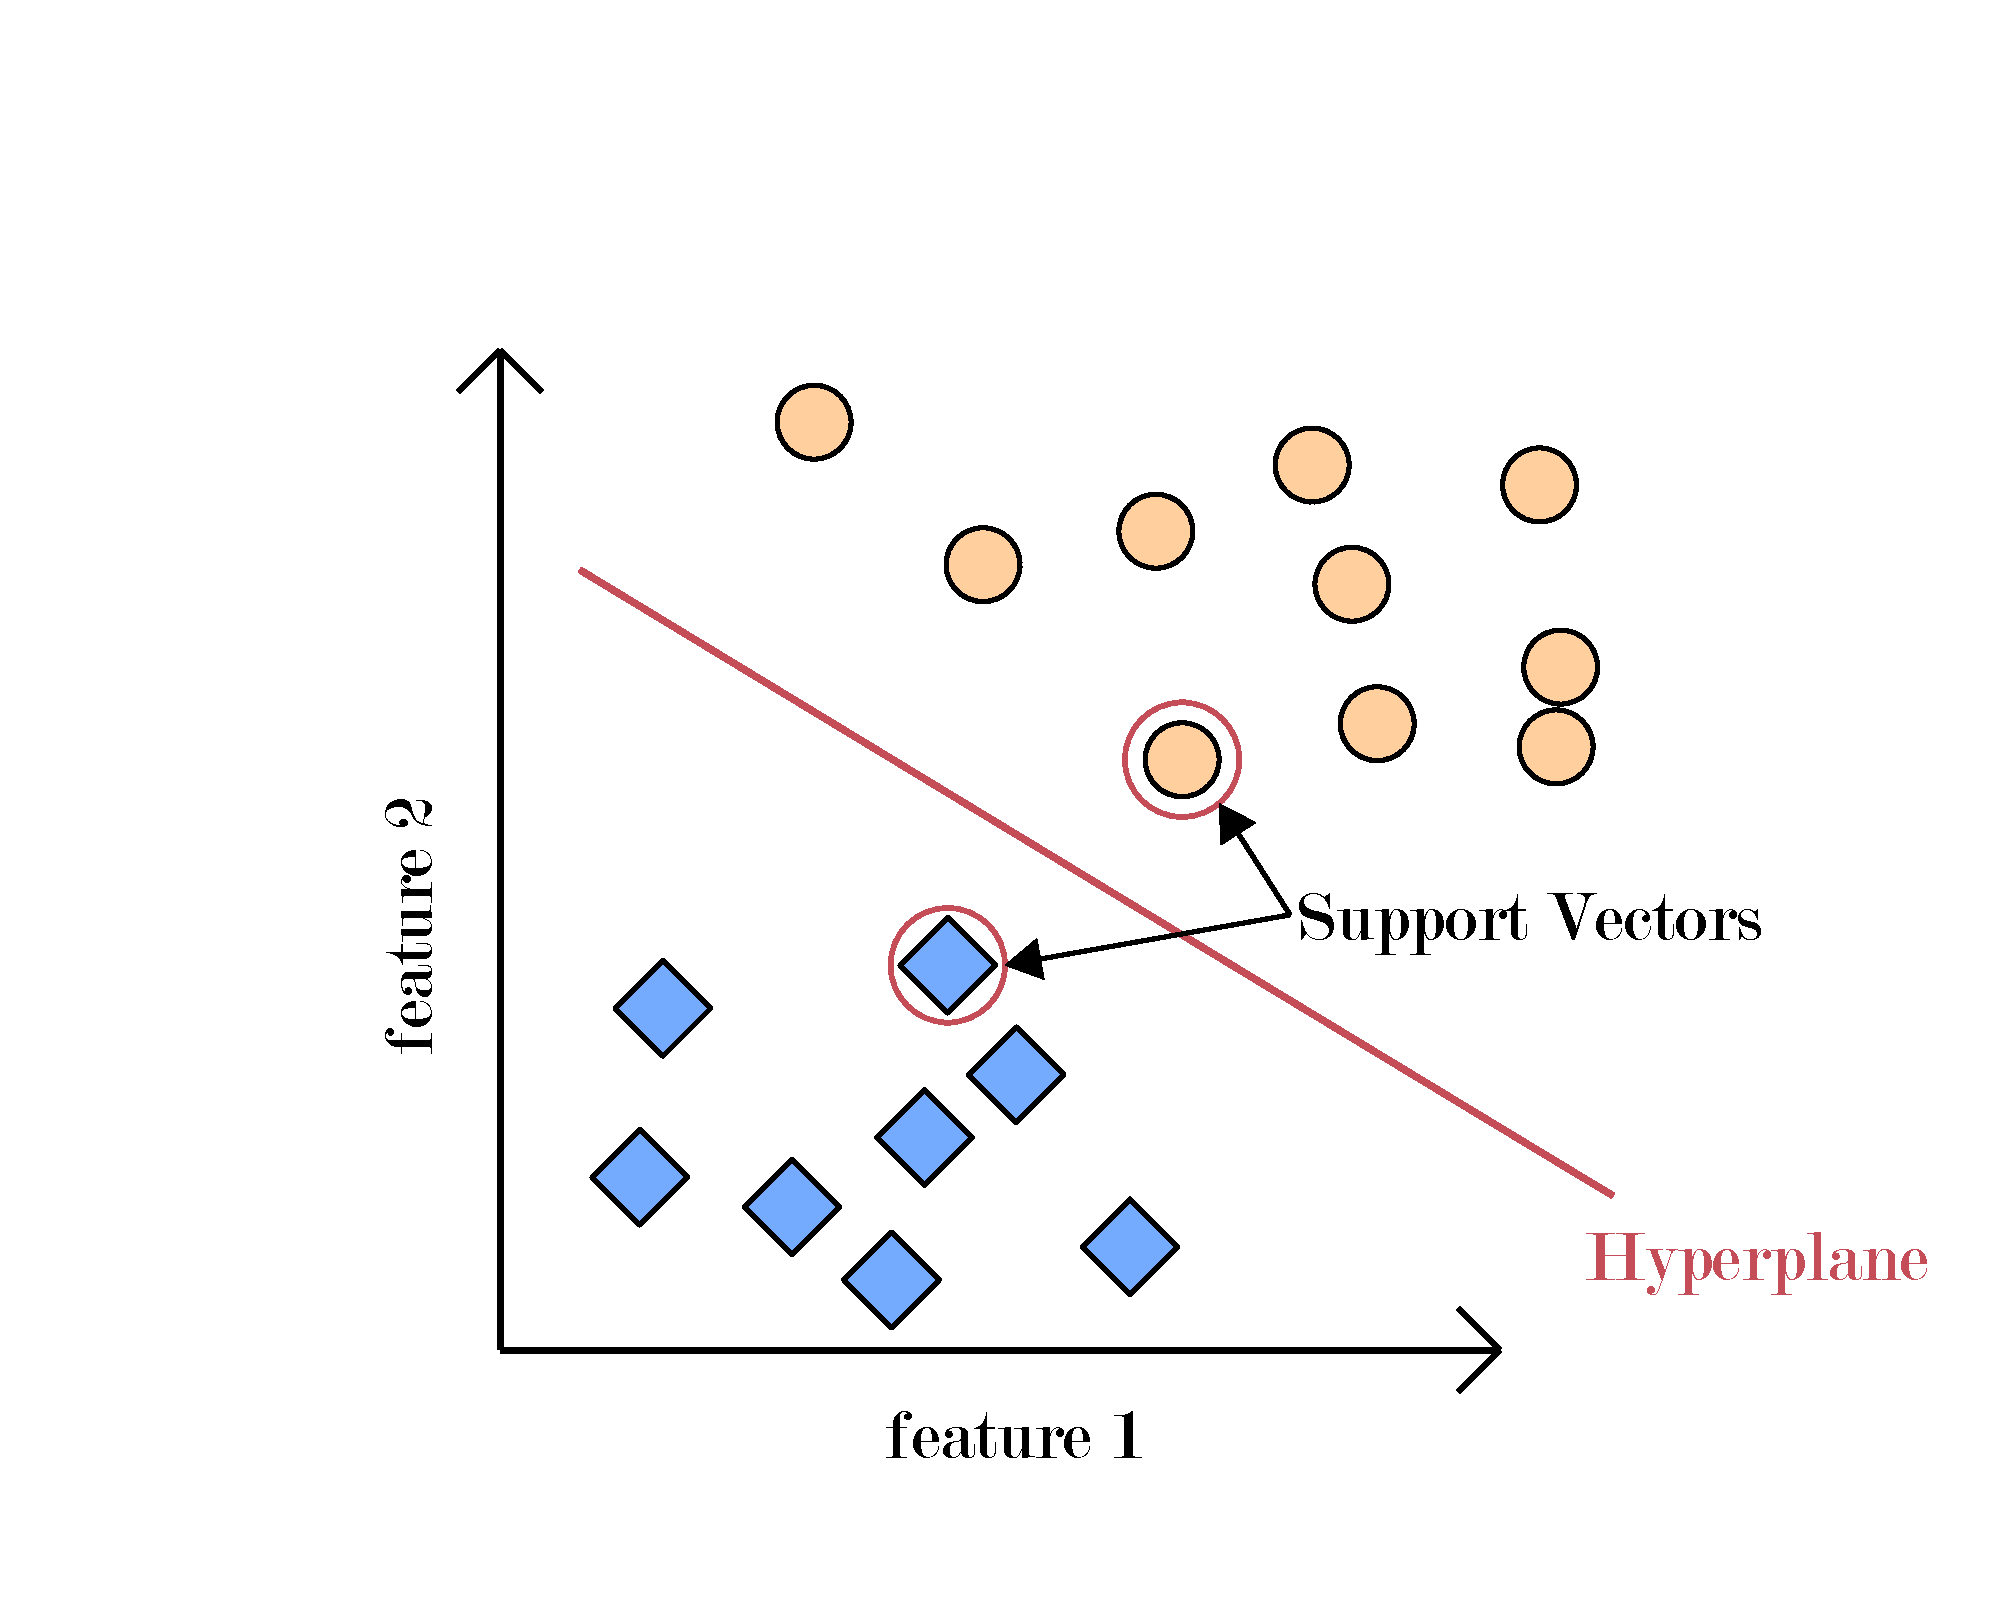
\includegraphics[width=0.6\columnwidth]{figures/support-vector-machines.pdf}
    \caption[Diagram of a Support Vector Machine]{Diagram of a Support Vector Machine}
    \label{fig:support-vector-machines}
\end{figure}
\FloatBarrier

\subsubsection{Long Short Term Memory (LSTM)}
Long Short Term Memory (LSTM - \autoref{fig:long-short-term-memory}) is a class of artificial neural networks. They are recurrent
networks meaning that data is not necessarily fed-forward as they allow for loops within the
network. LSTMs contain cells with `gates' that allow them to keep context and control the flow of data,
as well as make decisions to keep or discard data in order to make predictions. It is an example of a supervised neural network as labelled data is used in training.

\begin{figure}[hbt!]
    \centering
    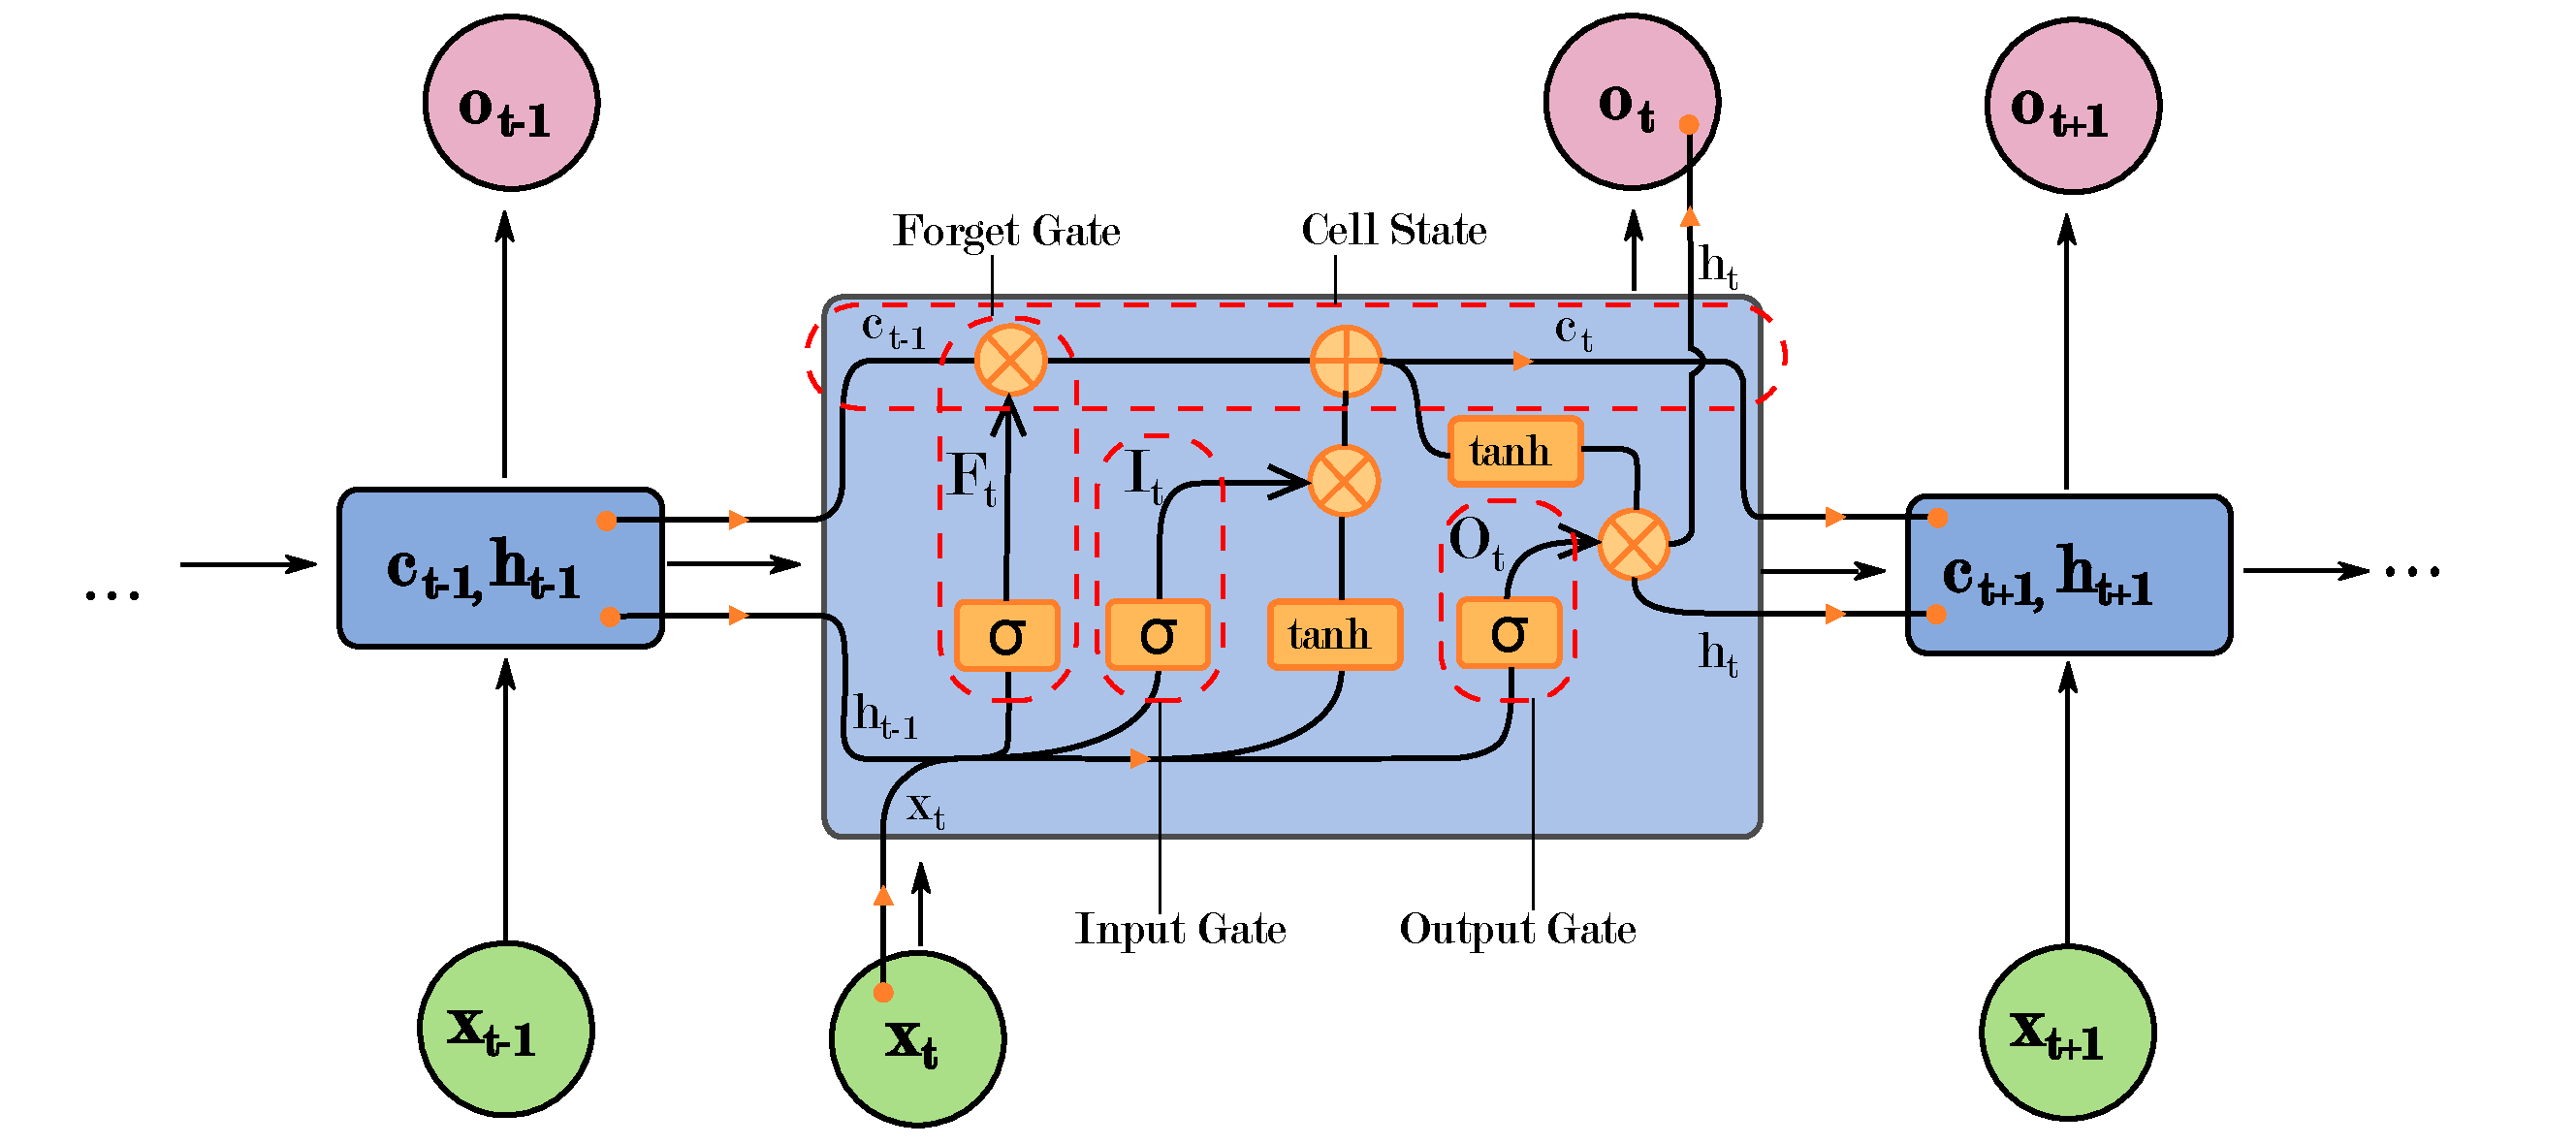
\includegraphics[width=\columnwidth]{figures/long-short-term-memory.pdf}
    \caption[Diagram of a LSTM Unit]{Diagram of a Long Short Term Memory Unitadapted from Long Short-Term Memory.svg, Wikimedia, fdeloche}
    \label{fig:long-short-term-memory}
\end{figure}
\FloatBarrier

\subsubsection{Hybrid Approaches}

Hybrid approaches can be utilised in order to overcome shortcomings in certain models. A hybrid
approach can utilise any number of different models; for example a CNN-LSTM hybrid model will use
CNN and LSTM layers as a CNN may be a good model for classification problems, an LSTM is better
suited to time series data.

\subsection{Artificial intelligence methods used in previous studies}

Different studies have utilised different artificial intelligence models to predict the price of stock market indices, with varying degrees of accuracy.

One study using multilayer perceptrons (MLP) to predict the daily direction of an exchange traded fund (ETF) that tracks the US S\&P 500 stock market index suggests that the model has an accuracy of up to 60\% \parencite{zhong2019predicting}. Whereas another study has suggested they can predict the price, not just direction, of the same stock market index with an accuracy of 76\% using support vector machines (SVMs) and reinforcement learning \parencite{shen2012stock}. As there is a difference of 16\%+ in of accuracy in the same stock market index (S\&P 500), and the higher accuracy model suggests that support vector machines may provide an improvement over feed-forward neural networks such as MLPs. Another study comparing the performance of MLPs and SVMs agrees that SVMs are superior as, even though both models were able to predict the direction of the S\&P 500 index, the MLP model had a maximum error difference of 15\% over a 45 day period, whilst the SVM model had a maximum error difference of 6\% in their test cases\parencite{comparisonregannsvm}. %interesting input features, mention in next part
This is further supported by another study comparing various artificial intelligence methods on the Indian Nifty50 index with the SVM model outperforming a back-propagation neural network model, which is somewhat similar to the MLP model, by 5.51\% \parencite{kumar2006forecasting}.

Further studies have been done on using hybrid approaches to predict stock markets. One study using an approach with a convolutional neural network (CNN) and three long short-term memory (LSTM) networks found that the accuracy of predicting weekly directions of the S\&P 500 index was 66.6\%, which was greater than with SVMs or CNNs alone,  with those models achieving 62.0\% and 59.3\% respectively \parencite{hao_gao_2020}. Another study agrees with these findings, with their results also suggesting a model built with CNNs and bi-directional LSTMs are able to outperform SVMs \parencite{noveldeepcnnbilstm}. However, the same cannot be said for all types of hybrid neural network models; one study comparing MLPs and hybrid networks on the US Nasdaq index has found that the MLP performs better, albeit slightly with a difference of 0.26\% in mean absolute deviation, than an approach with a hybrid model of MLP and Generalized Auto-Regressive Conditional Heteroskedasticity (GARCH) \parencite{GURESEN201110389}.

\section{Input features for intelligence methods}
The studies mentioned in the previous section use different input features for their studies; where the amount of input features ranges from just a single type of input to many various macro-economic factors. One of the hybrid approaches has only stated using the `daily closing price dataset of the S\&P 500 index' in their CNN-LSTM model \parencite{hao_gao_2020}. Another study using the hybrid approach slightly expands on this by using additional factors related to the index: the opening and closing prices of the S\&P 500 index, the low and high prices of the day, and the trading volume. However, these studies have not considered any macro-economic factors. One study expands on this further by also including other indexes across the world as inputs, as well as various currency rates in addition to commodities such as oil and metals \parencite{shen2012stock}. Other studies expand on this further, for example one study with 27 input features also includes US Treasury yield rates and bond yields \parencite{comparisonregannsvm} and another looks into additional factors for a total of 60 input features including certificate of deposit rates, and term and default spreads \parencite{zhong2019predicting} - though the latter study explains that with principal component analysis, the model peaked in terms of accuracy with 31 input features.

\section{Conclusion}
To conclude, there are differing opinions on whether or not markets are efficient, and therefore whether or not they are predictable. Some economists use the fact that experienced fund managers are rarely able to beat the market as proof that markets are efficient, and there are studies that agree with this hypothesis. However, there are also other studies that disagree presenting their findings that show there is some evidence of market inefficiencies in either the short term or long term.

Regardless of markets being efficient or not, numerous artificial intelligence methods -- including MLPs, SVMs, CNNs as well as hybrid approaches using CNNs and LSTMs -- have been employed to varying degrees of success. While some studies look at predicting just the direction, and others attempt to predict the price, most have claimed to be able to do so with above 50\% accuracy. From the studies researched here, it can be assumed that in general hybrid approaches involving CNNs and LSTMs outperform SVMs, which outperform MLPs.

These studies use a diverse set of input features in order to build their models, with some using features only directly related to the index and some using extended datasets including inputs from macroeconomic sources in order to build models that take account external factors that may affect the index's price, though there is evidence to suggest that not all of the input features are required to build a good model to predict the price of an index.